\documentclass{article}

\usepackage{graphicx}   % for graphics
\usepackage{subcaption} % for subplots
\usepackage{rotating}   % for landscape figure

% Input
%------------------------------------------------------------------------------
% path to figures directory
\newcommand{\FiguresDirnew}{./results/normal_void_to_absorber_2d/images}

% time discretization: "FE" or "SSPRK33"
\newcommand{\Discretization}{FE}

% type of figure: "figure" for portrait or "sidewaysfigure" for landscape
\newcommand{\FigureType}{sidewaysfigure}
%------------------------------------------------------------------------------

\begin{document}

\begin{\FigureType}[h]
   \centering
   \begin{subfigure}{0.3\textwidth}
      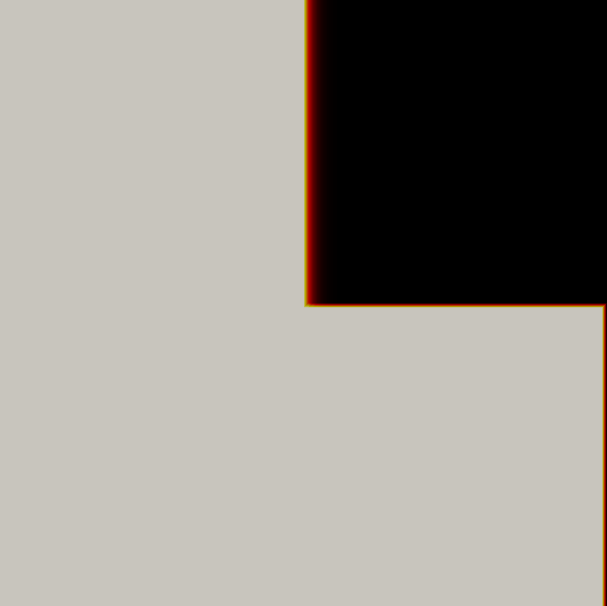
\includegraphics[width=1.0\textwidth]{\FiguresDir/Exact.png}
      \caption{Exact}
   \end{subfigure}
   \ifthenelse{\equal{\Discretization}{SSPRK33}}{
     \begin{subfigure}{0.3\textwidth}
        \includegraphics[width=1.0\textwidth]{\FiguresDir/Gal_\Discretization.png}
        \caption{Galerkin}
     \end{subfigure}
   }{}
   \begin{subfigure}{0.3\textwidth}
      \includegraphics[width=1.0\textwidth]{\FiguresDir/Low_\Discretization.png}
      \caption{Low-order}
   \end{subfigure}
   \begin{subfigure}{0.3\textwidth}
      \includegraphics[width=1.0\textwidth]{\FiguresDir/EV_\Discretization.png}
      \caption{EV}
   \end{subfigure}
   \begin{subfigure}{0.3\textwidth}
      \includegraphics[width=1.0\textwidth]{\FiguresDir/GalFCT_\Discretization.png}
      \caption{Galerkin-FCT}
   \end{subfigure}
   \begin{subfigure}{0.3\textwidth}
      \includegraphics[width=1.0\textwidth]{\FiguresDir/EVFCT_\Discretization.png}
      \caption{EV-FCT}
   \end{subfigure}
   \caption{Comparison of solutions with 16384 cells for the normally-incident
     absorber test problem using \Discretization{} time discretization}
\end{\FigureType}

\end{document}
